\section{Background and Related Work}\label{sec:background}

%% In this section, we introduce the concepts and terminology that are necessary to understand the reminder of this paper. First, Section~\ref{sec:sand} introduces some background information about \emph{sandboxes} within the security context. Section~\ref{sec:repackage} presents background information about repackaged application and how they introduce malicious behavior.
%% Finally, in Section~\ref{sec:android-sandbox} we review the \emph{mining sandbox approach} for detecting repackaged Android apps.

The Android bytecode language~\cite{DBLP:conf/issta/WangGMC15} favors reverse engineering tasks. That is, software developers can easily reverse-engineer real apps (benign), modify their contents by inserting malicious code (malware), repackage them with the malicious payloads, and re-publish them in app stores, including the Google Play Store. Repackaged Android apps can leverage the popularity of real apps, to increase its propagation and spread malware.  
Repackaging has been raised as a noteworthy security concern in Android ecosystem by stakeholders in the app development industry and researchers. Indeed, there are reports claiming that about 25\% of Google Play Store app content correspond to repackaged apps~\cite{DBLP:conf/sigmetrics/ViennotGN14}. Nevertheless, all the workload to detect and remove malware from markets by the stores (official and non-official ones), have not been accurate enough to address the problem. As a result, repackaged Android apps threaten security and privacy of unsuspicious Android app users, beyond compromising the copyright of the original developer~\cite{DBLP:journals/access/KimLCP19}. Aiming at
mitigating this threat, several techniques based on both static and dynamic analysis of Android apps have been proposed.

\subsection{Dynamic and Static Analysis on Android apps}\label{sec:analysis}

\todo[inline]{Handrick, we are not citing here the main research contributions in the area. I mean, is there any particular reason for citing the works in this section, instead of for instance FlowDroid? FlowDroid is by far one of the most relevant static analysis tools for analysing Android apps. Lets discuss how to rewrite this section here. I would suggest Handrick read these surveys, and then summarize this discussion highlighting the most relevant research works.

  \url{https://dl.acm.org/doi/pdf/10.1145/3017427}

  \url{https://ieeexplore.ieee.org/abstract/document/9118907}
}

{\color{red}
There is a large body of knowledge exploring the use of program analysis techniques to detect Android malware. 
Some of the designed techniques analyze the calls to sensitive methods or app's permission request
patterns~\cite{DBLP:conf/mobicom/WeiGNF12,DBLP:conf/asiajcis/WuMWLW12,DBLP:conf/sp/LiDLDG21}.
For instance, Au el al.~\cite{DBLP:conf/ccs/AuZHL12} statically analyze Android Manifest files to detect vulnerabilities in Android apps.
Their approach reasons about the permissions requested to sensitive API {\color{blue}in order to \ldots}. 
Kim et al. present RomaDroid~\cite{DBLP:journals/access/KimLCP19}.  Their approach treats the app code as
sequence of strings and then tries to identify repackaged apps using the lowest common subsequence (LCS) algorithm. 
%At our work we also apply static analysis but not on Manifest files. At your investigation we try to find suspicious code just at Android bytecode. % \kn{How is this approach different from ours? }

Li et al.~\cite{DBLP:journals/tifs/0029LBKTLC17} provide a taxonomy of Android malware, built upon an indepth empirical study that compares malicious repackaged apps with their benign counterparts (1,497 app pairs). They found that the majority of Android malware are repackaged versions of benign apps that do not perform any complex modification. Also in the domain of detecting repackaged apps by comparing app pairs, Crussell et al.~\cite{DBLP:conf/esorics/CrussellGC12} proposed  DNADroid, which compares program dependence graphs, and Zhou et al.~\cite{DBLP:conf/codaspy/ZhouZJN12} proposed DroidMoss, which detects and analyzes repackaged apps using a fuzzy hashing technique. The insights from the above mentioned works re-emphasize the need to ensure approaches that work on detecting repackaged apps with a good accuracy. 


% \todo[inline]{It seems to me the following research works do not relate to our research. Is there any particular reason for citing them?}

Cai et al.~\cite{DBLP:journals/tse/CaiR21} present
a longitudinal study on Android apps focusing on run-time behaviors. However, this work does not focus specifically on malware detection but on general security gaps in apps by considering only benign apps. Fangfang et al.~\cite{DBLP:conf/wisec/ZhangHZW014} proposed ViewDroid, which models the UIs of Android apps as a directed graph. Although ViewDroid also works by comparing app pairs to identify repackaged apps, their focus is UI centric.
}
\subsection{Mining Android Sandboxes}\label{sec:android-sandbox}

A \emph{sandbox}
is a well-known mechanism to secure a system and forbid a software component from accessing
resources without appropriate permissions. Sandboxes have also been used to build an isolated
environment within which applications cannot affect other programs, the network, or other device data~\cite{DBLP:journals/peerj-cs/MaassSCS16}. The idea of using sandboxes emerged from the
need to test unsafe software, possible malware, without worrying about the integrity of the
device under test~\cite{DBLP:conf/esorics/BordoniCS17}, shielding the operating system from security issues.
To this end, a sandbox environment should have the minimum requirements to run the
program (make sure the program will not spill out of the sandbox), and make sure it will never
assign the program greater privileges than it should have, respecting the principle of
\emph{least privilege}. This principle ensures unauthorized access to resources,
improving the system's overall health. Within the Android ecosystem, sandbox approaches ensure the principle
of the \emph{least privilege} is ensured by preventing apps from having direct access to resources or data from other apps. Access to sensitives resources
like contacts list is granted through specific APIs (Application Programming Interface),
which are managed by permissions system~\cite{DBLP:journals/corr/abs-2109-06613}. 

%% The main market source for Android apps is Google Play Store. Unfortunately, it has
%% a flexible policy regarding the process of publishing apps, and therefore, many Android apps are removed from the
%% store because of issues related to malware\cite{DBLP:conf/msr/WangLL0X18}. Google Play tries
%% to minimize unauthorized access to sensitive resources by malicious apps,
%% listing each app with its requested permission. {\color{red}Those permissions are presented to Android
%% users at app installation moment since version 6}. However, some works presented that most users are careless regarding these permissions since they are only interested to run the app~\cite{DBLP:conf/soups/FeltHEHCW12}. This represents a great security breach since malware usually asks for more permissions than their APIs normally would require~\cite{DBLP:conf/ccs/FeltCHSW11}.



The Mining Android Sandbox approach~\cite{DBLP:conf/icse/JamrozikSZ16} aims at automatically
building a sandbox through dynamic analysis (i.e., using automatic test generation tools).
The main idea is to explore apps based on their calls to sensitive APIs.
Thus, sandboxes build upon these calls to create safety rules and then block future
calls to other sensitive resources, which diverge from those found in the first exploratory
phase. Using a test generation tool named Droidmate~\cite{DBLP:conf/icse/JamrozikZ16},
Jamrozik et al.~\cite{DBLP:conf/icse/JamrozikSZ16} proposed a full fledged
implementation of the Mining Android Sandbox approach, named Boxmate. 
Boxmate records the occurrences of calls to sensitive APIs and the UI events that triggers these calls,
like a button click. It is possible to configure Boxmate to record events associated with each sensitive call as
tuples (event, API), instead of recording just the set of calls to sensitive APIs. Jamrozik et al. argue that, in this way, Boxmate generates finer granularity results which
might reduce false alarms, even with the presence of reflection which is quite commonly used in
malicious apps~\cite{DBLP:conf/issta/0029BOK16}.

In fact, the mining sandbox approach can be implemented using
a mix of static and dynamic analysis. In the first phase, one
can instrument an Android app to log any call to the Android sensitive methods.
After that, one can execute a test case generation tool (such as DroidBot
or Monkey) to explore the app behavior at runtime,
while the calls to sensitive APIs are recorded.
Figure~\ref{fig:mineSandbox} presents this general approach for mining
Android sandboxes. This set of calls to sensitive APIs is then used
to configure the sandbox. 

\todo[inline]{Since this figure is not discussed in the paper, we can remove it without any problem. I have enriched the previous paragraph, though, to make it
  more necessary. Nonetheless, I will change this figure a bit, in order to
represent the instrumentation phase.}

\begin{figure}[ht]
\centering
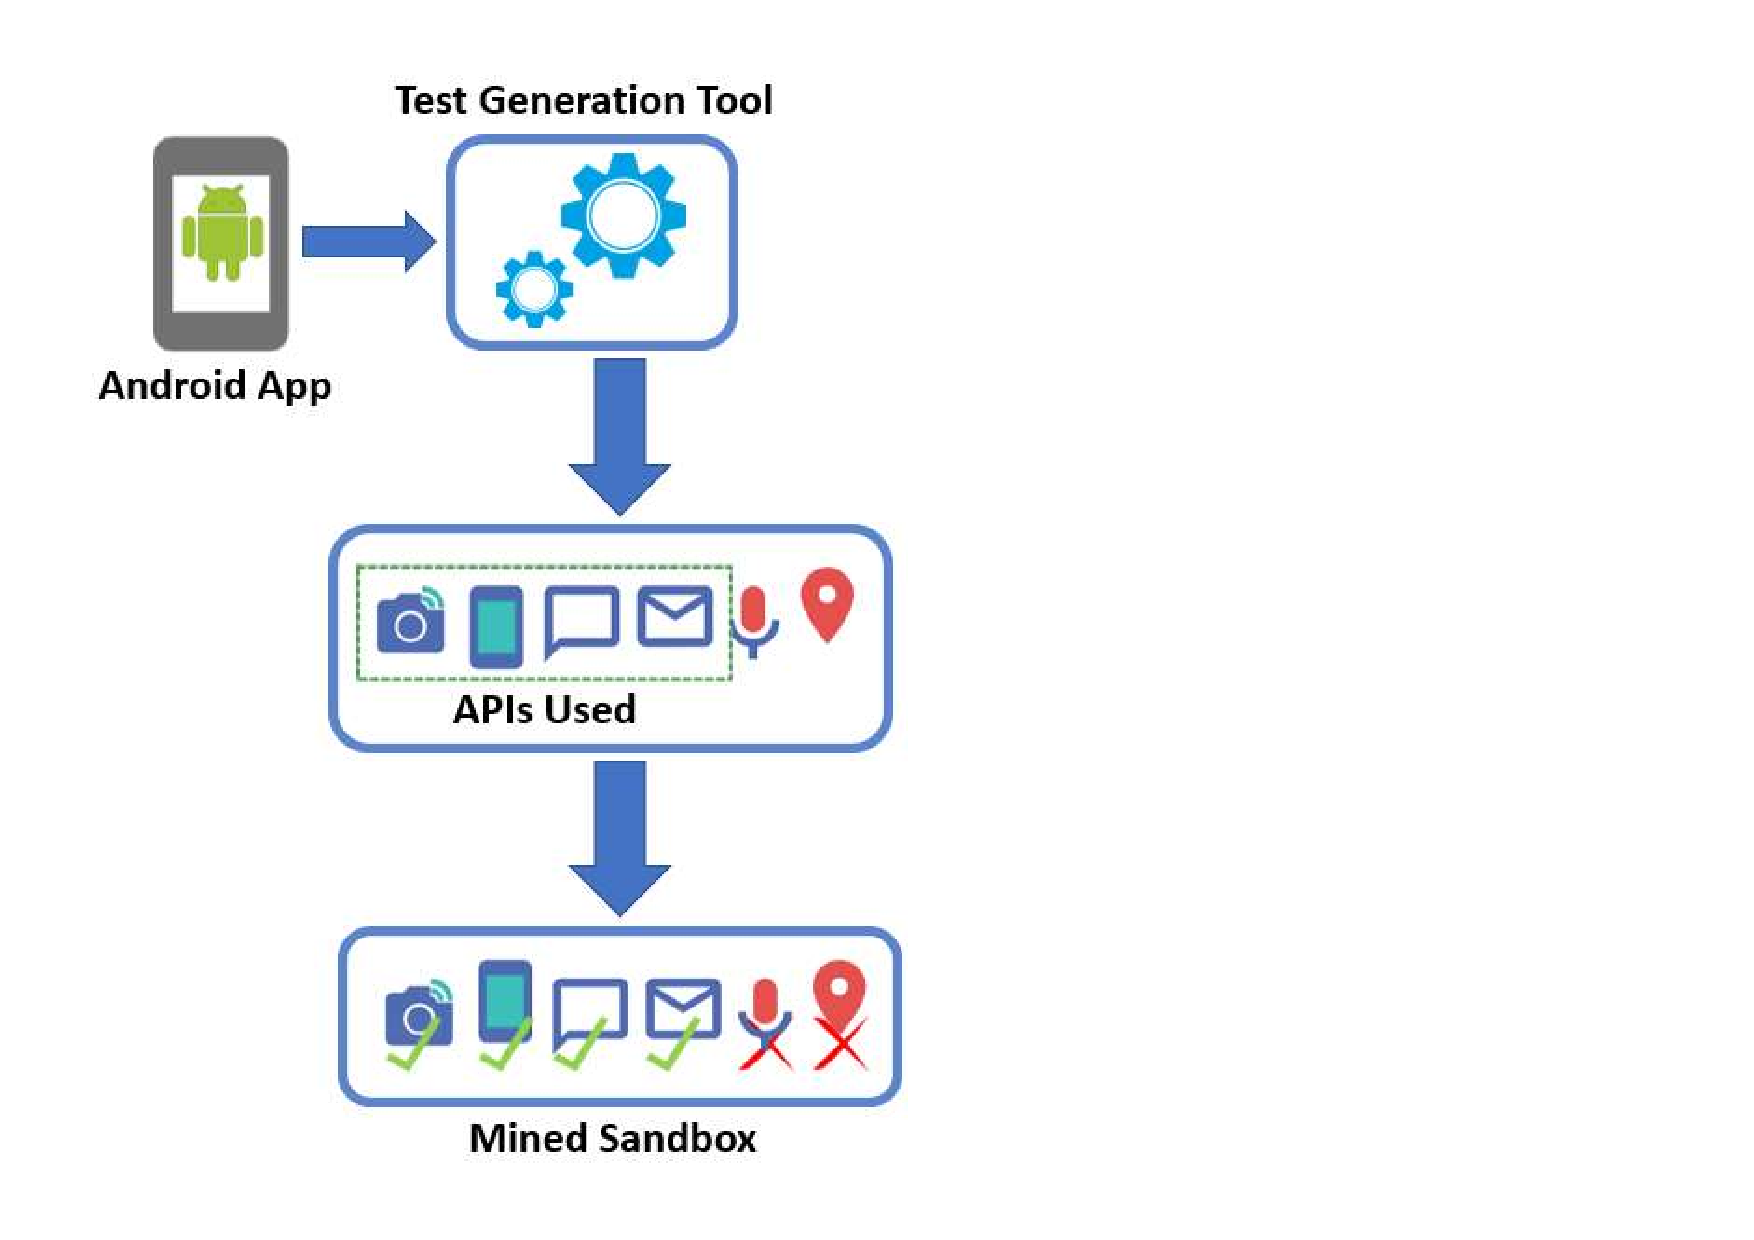
\includegraphics[scale=0.35]{images/mineSandbox_.pdf}
\caption{Mine Sandbox.}
 \label{fig:mineSandbox}
\end{figure}

\subsection{Mining Android Sandbox for Malware Identification}

Besides being used to generate Android sandboxes, the Mining Android Sandbox approach is also effective 
to detect Android apps with suspicious behaviors~\cite{DBLP:conf/wcre/BaoLL18}.  In this scenario, the \emph{effectiveness} of the approach
is estimated in terms of accuracy in which repackaged apps are identified.
The general mining sandbox approach (see Figure~\ref{fig:mineSandbox}) suggests
that the more efficient the test generator tool (for instance, in terms of code coverage),
the more accurate would be the resulting sandbox.


Figure~\ref{fig:sensitiveAPI} illustrates the Mining Android Sandbox approach for
repackaged apps identification. We leverage DroidXP to collect the set of sensitive APIs the versions of the apps call (benign/malign versions). As a first step, given one benign app version,
our approach first collects all calls to sensitive APIs from the app code through static analysis. Then, during the execution step,
we use dynamic analysis to collect all calls to sensitive APIs during the DroidBot test case execution. We configure DroidXP to execute DroidBot for a
period of $3$ minutes. Since some malicious app may use dynamic features (such as reflection) to introduce malicious behavior, which can change the behavior of the apps at runtime~\cite{DBLP:journals/spe/ZhangLTX18,DBLP:journals/tosem/LiTX19}, this second analysis is also important to disclose some sensitive APIs calls ignored by static analysis.

While our static analysis is made once, we execute dynamic analysis $3$ times. The result of static analysis and all executions is finally joined, forming a final set that contains all identified calls to sensitive APIs coming from the benign version of the app, as described at Figure~\ref{fig:sensitiveAPI}: ($S_{A}$, $D_{A1}$, $D_{A2}$, $D_{A3}$). We carry out the same procedure for the malicious version of the apps,
creating a distinct set of calls to sensitive APIs (now coming from the malicious version of the apps). In
a final step, we compare the two sets of calls to sensitive APIs ($Set_B, Set_M$). We use the following rules to
check for a malicious behavior. 

\begin{enumerate}
    \item If the difference between the two final sets is an empty set, we cannot distinguish the benign from the malicious version of the app (false negative).
    \item Otherwise, we successfully distinguish the benign from the malicious version of the app (true positive). 
    %\kn{Cant we replace the first part of the second point simply as "Otherwise" or is there some specific corner cases that I am missing}
\end{enumerate}

In addition, this procedure also enables us to identify the calls to sensitive APIs that are more frequently injected by the malicious version of the apps
in our dataset. 

%\fh{here I have to insert the figure}

\begin{figure}[ht]
\centering
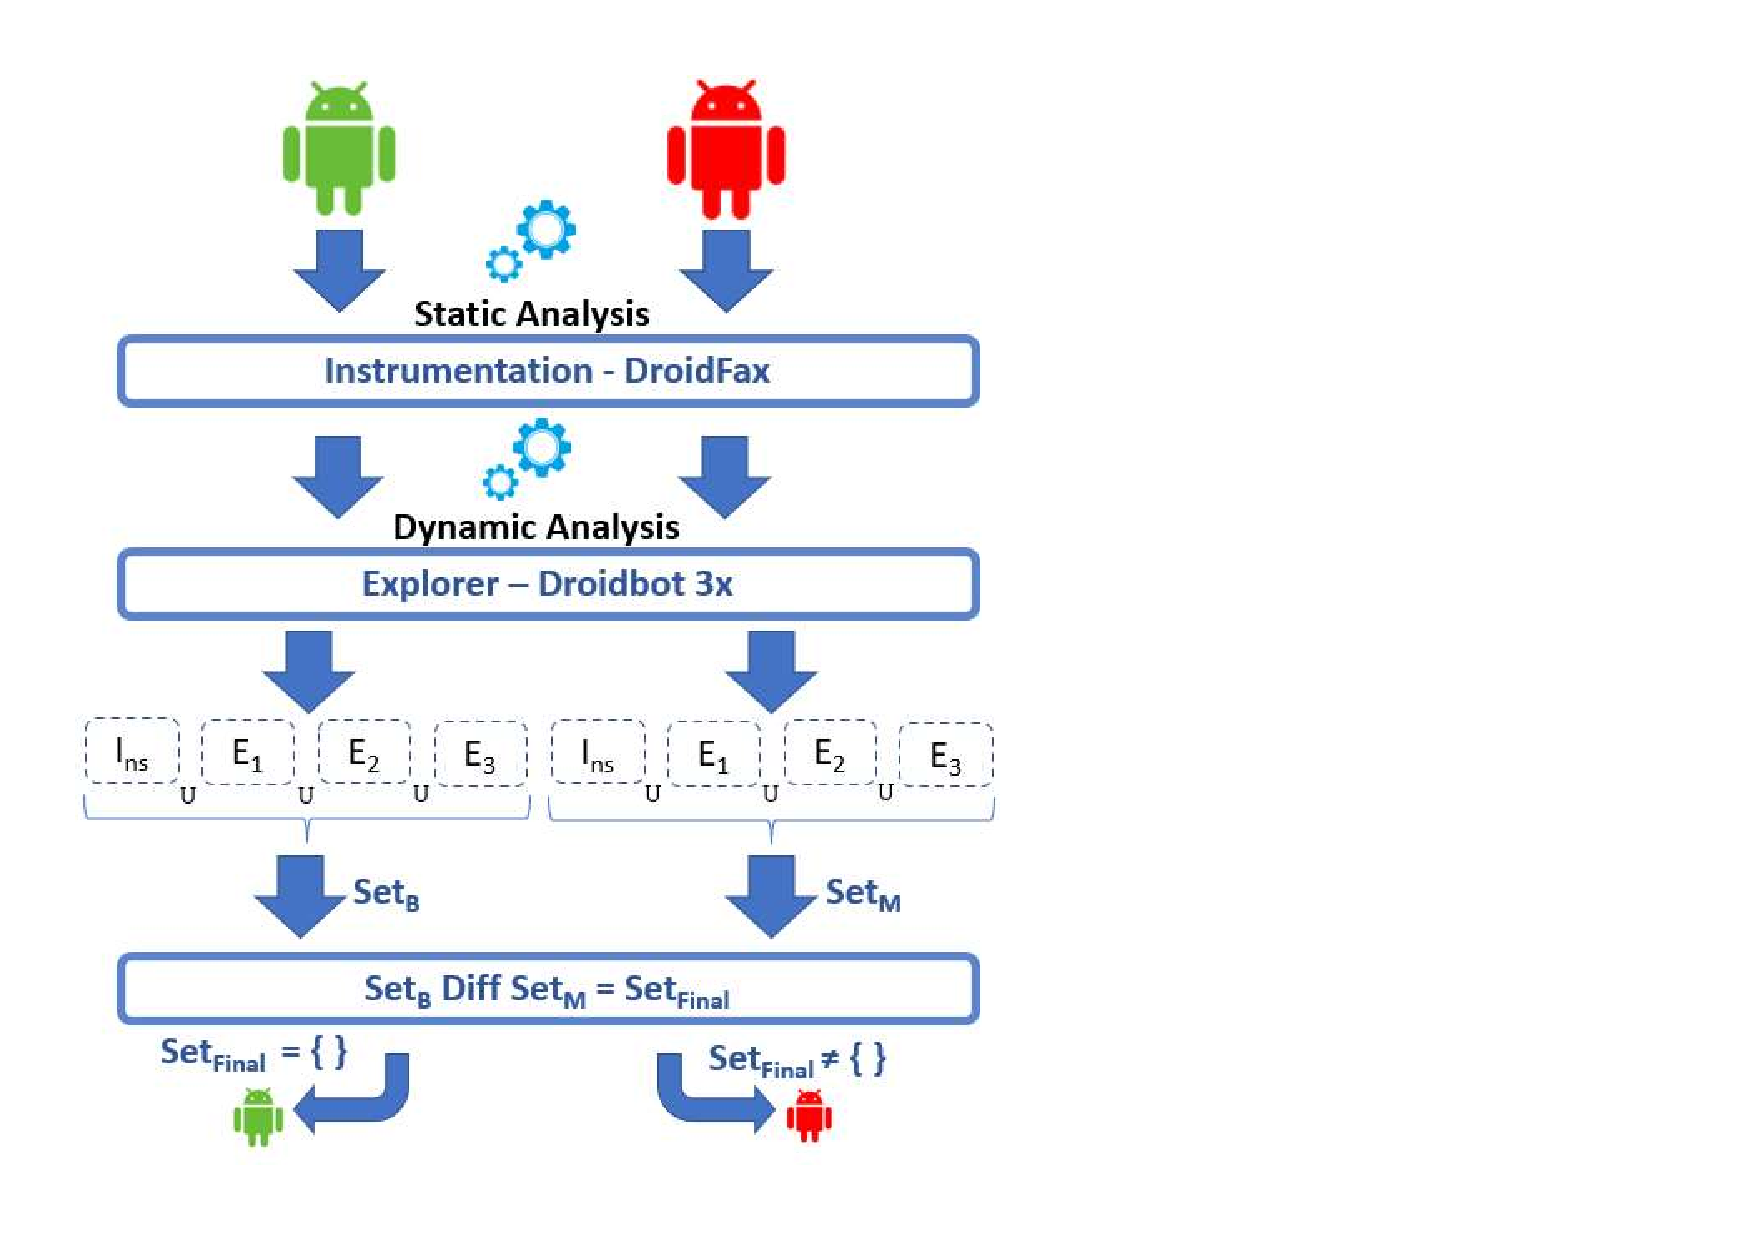
\includegraphics[scale=0.45]{images/sensitiveAPIdiff.pdf}
\caption{All procedure for suspicious app identification using sensitive API set diff.}
 \label{fig:sensitiveAPI}
\end{figure}



%\kn{I have commented out the subsection here as it seems redundant with the previous subsection}
%\subsection{The Mining Android Sandbox Approach for Malware Identification}

%The focus of our paper is in approaches that mine android sandboxes to classify Android Malware.
%There is a vast body of research in this direction. 

Costa et al. and and Bao et al.~\cite{DBLP:conf/wcre/BaoLL18,DBLP:conf/scam/CostaMCMVBC20} conducted empirical studies to investigate the effectiveness of Mining Android Sandbox
approaches, exploring test generation tools, including DroidBot. These works served as base for our investigation and\rb{our goal is not to: , consequently for negative result discovery}. Bao et al. found that, in general, the sandboxes constructed using test generators can detect more than $66$\% malicious apps in a dataset comprising $102$ pairs (benign/malicious). The study also presented that among $5$ test generation tools used, DroidBot~\cite{DBLP:conf/icse/LiYGC17} is the most effective sandbox.
Le et al.~\cite{le2018towards} extend the work of Bao et al. by combining more categories of sensitive APIs, and also considering the impact of actual parameters, combining sensitive APIs calls and input parameters of these APIs.
%\kn{What arguments? function parameters?}. 
Costa et al.\cite{DBLP:journals/jss/CostaMMSSBNR22} investigated the impact of static analysis to complement the accuracy of dynamic analysis tools for mining sandboxes. The study found that DroidFax~\cite{DBLP:conf/icsm/CaiR17a}, the static analysis infrastructure used in~\cite{DBLP:conf/wcre/BaoLL18}, is able to detect almost half of repackaged apps in a
dataset of $96$ pairs of benign/malicious apps.

%\todo[inline]{I could not understand why we did not cite our JSS work here}
%However, none of the aforementioned studies
% ~\cite{DBLP:conf/icse/JamrozikSZ16,DBLP:conf/wcre/BaoLL18,le2018towards}
%neither characterize the APIs included on the repackage versions nor investigate the
%possibility that trace analysis using call graph or analysis of
% the manifest file could complement the mining sandbox approach for malware identification.

\subsection{Extending the Mining Sandbox with Trace Analysis}

Our work, although closely related to previous studies, differs from them in several aspects.  First, our assessment is more comprehensive: instead of considering $102$ pairs of benign/malign apps, we execute our study considering $1204$ pairs of apps. Curiously, the performance of the mining sandbox approach in our large dataset drops significantly. We then investigate which characteristics of the malware samples in the large dataset explain the lower performance we observed and also explore an extension to the malware sandbox approach that compare the traces from the app entry points to the calls to sensitive APIs, considering the benign and malign versions of the apps. 

As we discussed in the previous section, we take advantage of DroidXPTrace to build the dynamic call graphs that characterize the execution of each version of the apps in our dataset. Our goal
here is to explore how many pairs of apps call the same set of sensitive APIs, though using different call
traces. We hypothesize that differences in the traces might be used to complement the Mining Android Sandbox approach for suspicious app identification. As such, here we execute the trace analysis for all app pairs of our dataset, and check if there are situations in which the basic version of the Mining Android Sandbox approach was not able to correctly classify the malign version of an app as a piggybacked, however it has a different execution trace. For detecting different trace, we performed an evaluation of the dynamic call graph of each pair. Our procedure checks if there is some new node, representing a new sensitive API at malicious version, or a new edge($x$, $y$), where $x$ and $y$ indicates a method $x$ calling a sensitive method $y$.

%\rb{(Not sure if this is the right decision. I do not see any problem in running
%  this study for all pairs.)}. 
%% we  investigate those app pairs that were not described as a malware during the exploratory step, i.e,
%% the test generation tool DroidBot collected the same set of sensitive APIs for both version. If a dynamic call graph
%% of these app pairs presented different traces from entry point to sensitive APIs call at both versions, we suspect this to indicate presence of malware.
Figure~\ref{fig:callGraph} illustrates an example of benign and malicious call graphs.
At this example, although both app versions access the same set of sensitive resources, the
malicious version follows a different execution trace. 


\begin{figure}[ht]
\centering
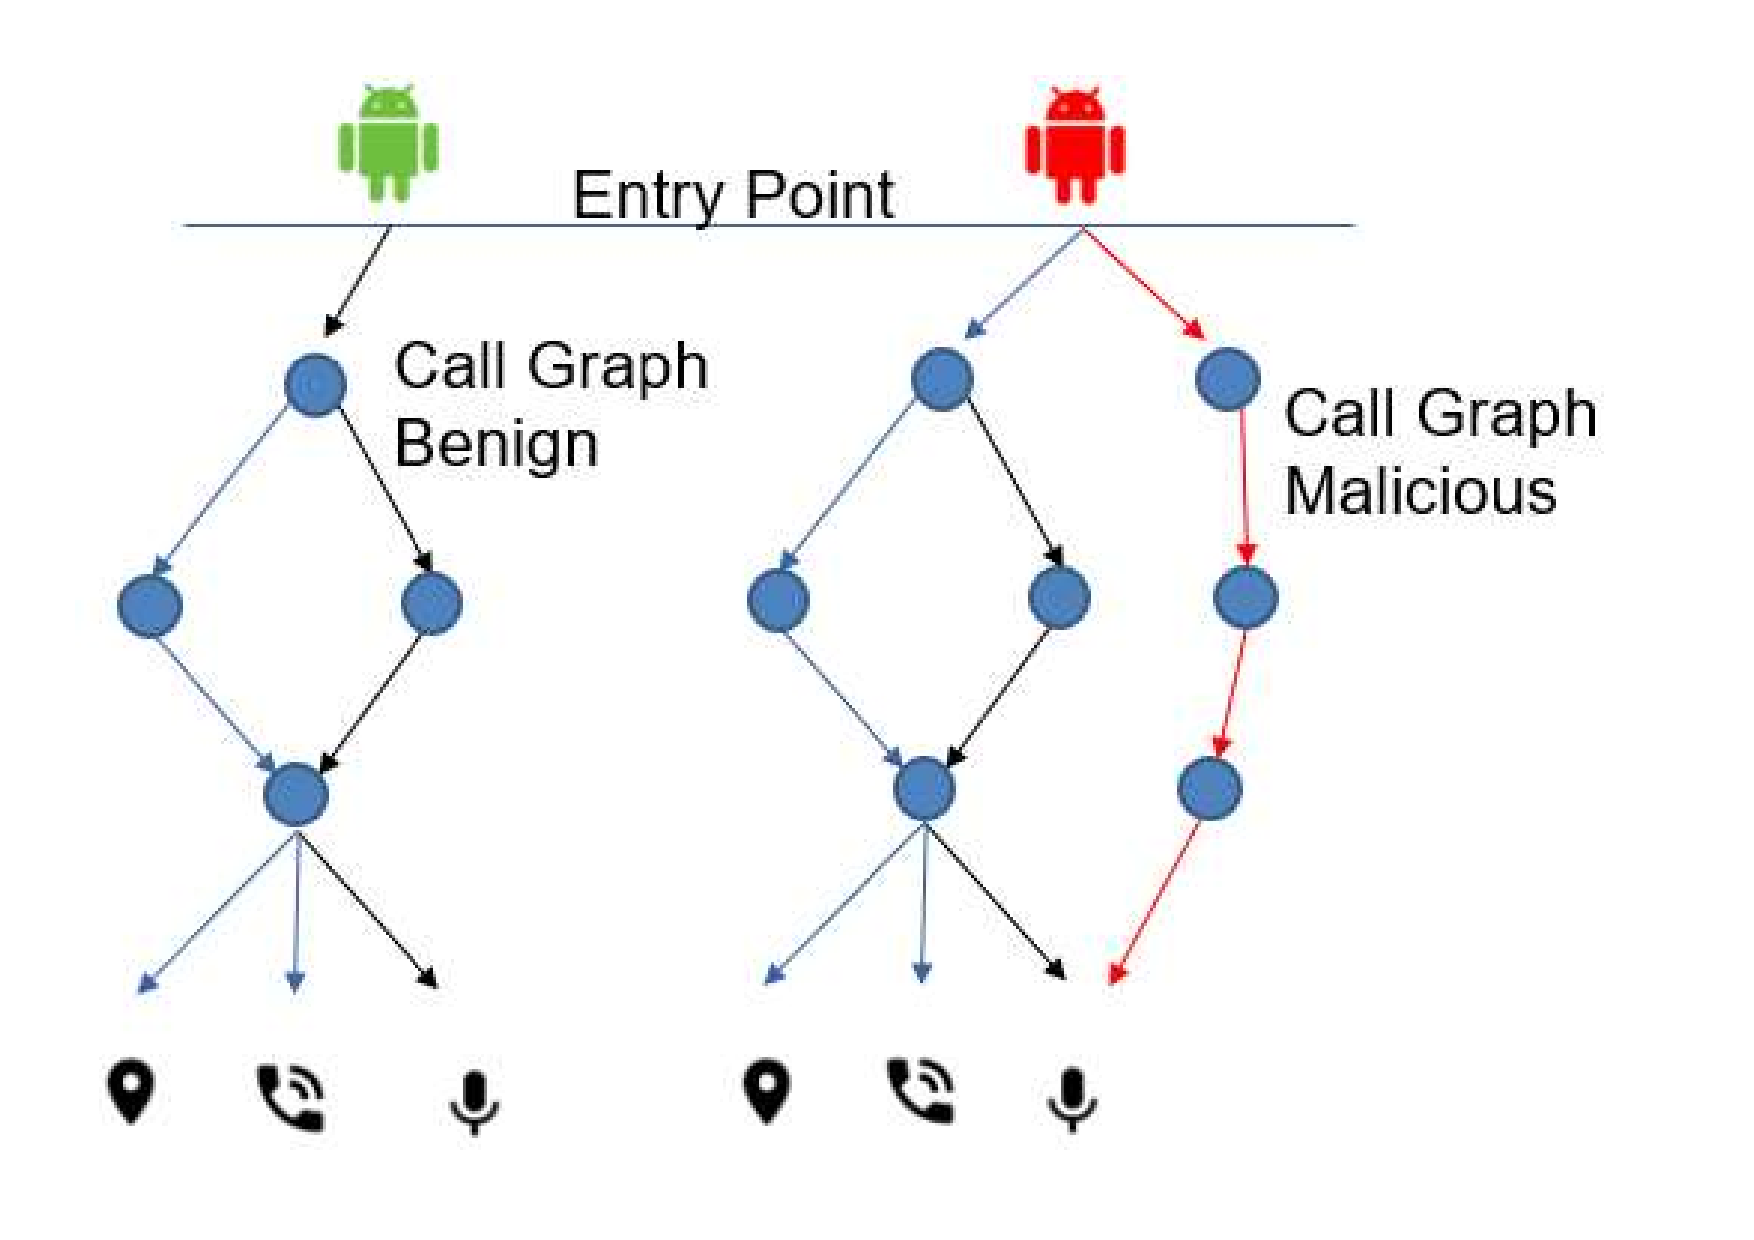
\includegraphics[scale=0.30]{images/maliciousCallGraph.pdf}
\caption{Illustrative example of the trace analysis. In this case, both versions call the same set of sensitive APIs. Nonetheless,
the traces between the entry point and the calls to sensitive APIs diverge.}
 \label{fig:callGraph}
\end{figure}

